%================================================================
%\chapter{The Bayesian Paradigm}\label{chap:bayesian}
\chapter{Bayesian Inference}\label{chap:bayesian}
%================================================================

\epigraph{A decision was wise, even though it led to disastrous consequences, if the evidence at hand indicated it was the best one to make; and a decision was foolish, even though it led to the happiest possible con-\\sequences, if it was unreasonable to expect those consequences.}{Herodotus, around 500 BC}


The aim of statistical inference is to learn about underlying properties of a population from observed data.  In statistical inference, there are, broadly speaking, two paradigms for the analysis of observed data: \textit{frequentist} inference and \textit{Bayesian} inference. These often differ with each other on the fundamental interpretation of probability. In the frequentist view, the probabilities of events are defined as their relative frequencies in a repeatable objective process, and are thus ideally devoid of opinion. From a Bayesian perspective, probabilities are measures that quantifies the uncertainty level of statements based on the degree of belief about the state of the world. Probabilities can be assigned to any statement, even when a random process is not involved. Bayesian inference is the process of revising beliefs about the state of the world in the light of new evidence.     

%The Bayesian view of probability, on the other hand, is based on the degree of belief about the state of the world, and probabilities can be assigned to any statement, even when a random process is not involved. Bayesian inference is the process of revising beliefs about the state of the world in the light of new evidence.   

%This chapter introduces the fundamentals of Bayesian inference, with a particular focus on parameter inference. The content of this chapter is mainly based on the material in the Bayesian textbooks \cite{BDA}, \cite{BAP} and \cite{Sivia}.

This chapter introduces the fundamentals of Bayesian inference, with a particular focus on parameter inference. The content of this chapter is based on the material in the Bayesian textbooks \cite{BDA}, \cite{BAP} and \cite{Sivia}.


%================================================================
%\section{Bayesian Inference}\label{sec:bayes_paradigm}
\section{Bayes' Theorem}\label{sec:bayes_paradigm}
%================================================================

In terms of parameter inference, the Bayesian approach differs from the frequentist in that unknown parameters $\theta$ are treated as random variables rather than fixed quantities. In the Bayesian paradigm, all available information about an unknown parameter is incorporated in a \textit{prior probability distribution}, expressing our beliefs before some evidence is taken into account. We usually have a prior pdf $\prior$, since there will typically be a continuum of possible values of a parameter rather than just a discrete set. In the case of substantial prior knowledge about a parameter $\theta$, the prior pdf is narrow and concentrated about some central value, whereas a lack of information yield a wider and relatively flat prior pdf as shown in \autoref{fig:prior_illustration}. The prior is often specified by a particular distribution among a set of well-known and tractable distributions, with the purpose of making evaluation of prior probabilities and random generation of $\theta$ values straightforward.

%In terms of parameter inference, the Bayesian approach differs from the frequentist in that unknown parameters $\theta$ are treated as random variables rather than fixed quantities. In the Bayesian paradigm, all available information about an unknown parameter is incorporated in a \textit{prior probability distribution}, expressing our beliefs before some evidence is taken into account. We usually have a prior pdf $\prior$, since there will typically be a continuum of possible values of a parameter rather than just a discrete set. In the case of substantial prior knowledge about a parameter $\theta$, the prior pdf is narrow and concentrated about some central value, whereas a lack of information yield a wider and relatively flat prior pdf as shown in \autoref{fig:prior_illustration}. The prior is often specified by a particular distribution among a set of well-known and tractable distributions (see \autoref{sec:Appendix A}), with the purpose of making evaluation of prior probabilities and random generation of $\theta$ values straightforward.

%\begin{figure}[H]
%    \centering
%    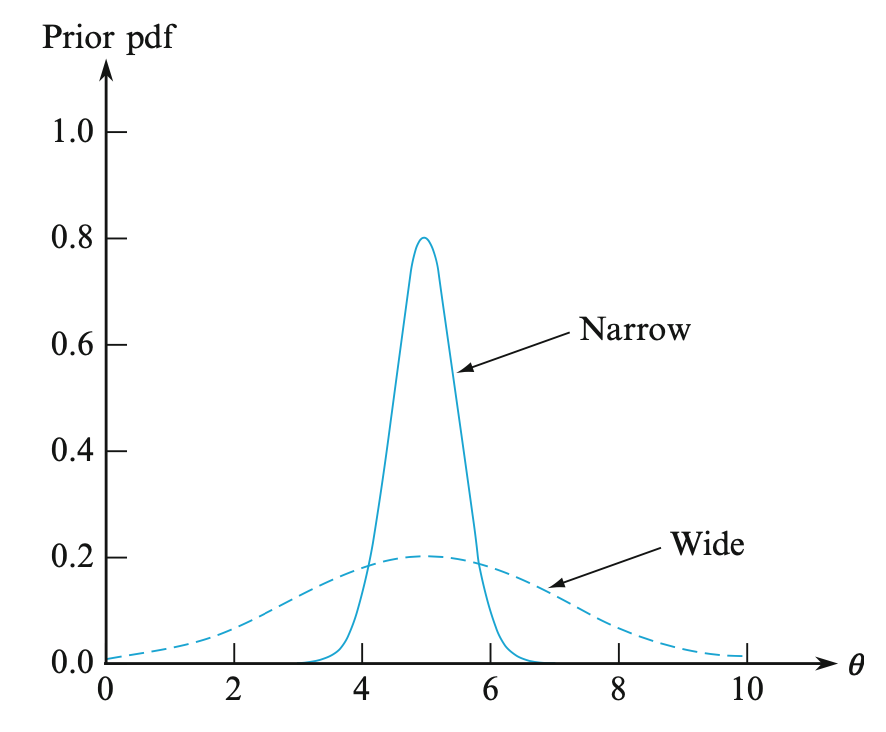
\includegraphics[scale=0.6]{./3_Images/prior_illustration.png}
%    \caption{A narrow concentrated prior about some central value and a wider less informative prior.}
%    \label{fig:prior_illustration}
%    \source{Figure 14.3 in \cite{STK}.}
%\end{figure}


\begin{figure}[H]
    \centering
    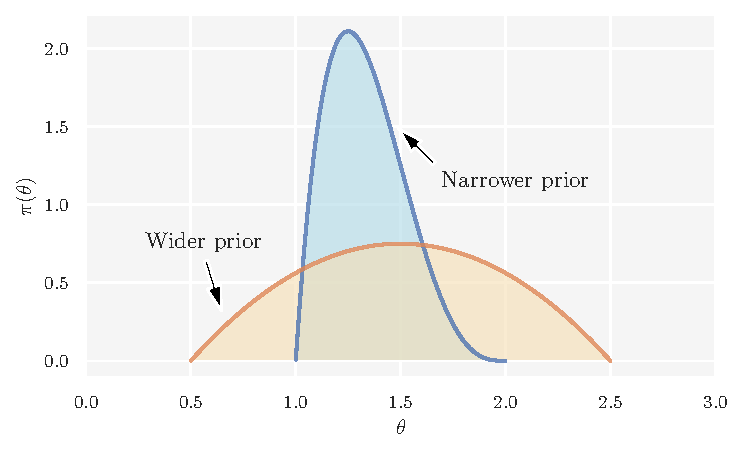
\includegraphics[scale=1.0]{prior_plot}
    \caption{Two prior distributions $\pi (\theta)$. A narrow concentrated prior (more certainty) about some central value and a wider less informative prior (less certainty).}
    \label{fig:prior_illustration}
    %\source{Figure 14.3 in \cite{STK}.}
\end{figure}

Our prior state of knowledge is modified by data $y$, obtained by performing experiments, through the conditional \textit{sampling distribution} $\lhood$. When regarded as a function of $\theta$, for fixed $y$, $\lhood$ is called the \textit{likelihood function}. In order to make probability statements about $\theta$ given sample data $y$, a probabilistic model representing the joint probability distribution for $\theta$ and $y$ must be provided. The joint pmf or pdf can be written as a product of the prior distribution $\prior$ and the likelihood function $\lhood$:

\begin{equation*}
    \joint = \lhood \prior .
\end{equation*}

At this point, Bayes' theorem is used to produce the \textit{posterior distribution}, which represents our state of knowledge about $\theta$ in the light of $y$. A common incarnation of Bayes' theorem is:

\begin{equation}\label{eq:bayes_theorem}
    \posterior = \frac{\joint}{p(y)}  = \frac{\lhood \prior}{p(y)},
\end{equation}

where the marginal probability of the data $p(y) = \int \lhood \prior \dd \theta$ in the case of continuous parameters, or, in the case of a discrete set of parameters, $p(y) = \sum_\theta \lhood \prior$, where the sum is over all possible values of $\theta$.

$p(y)$ is the same for all possible $\theta$, as it does not depend on $\theta$. With fixed $y$, this factor can thus be omitted in parameter inference since it constitutes a normalizing constant and does not enter into determining the relative posterior probabilities of different values of $\theta$. Omitting the factor $p(y)$ yields the unnormalized posterior distribution: 

\begin{equation}\label{eq:bayes_unnorm}
    \posterior \propto p(\theta, y) =  \lhood \prior .
\end{equation}

In this formulation, $\lhood$ is taken as a function of $\theta$ and not $y$.  

The core of Bayesian inference is encapsulated in \autoref{eq:bayes_theorem} and \autoref{eq:bayes_unnorm}. The principal task is to develop the joint probability model $\joint$ and perform the computations to obtain the posterior $\posterior$.

%The core of Bayesian inference is encapsulated in \autoref{eq:bayes_theorem} and \autoref{eq:bayes_unnorm}. The principal task is to develop the joint probability model $\joint$ and perform the computations to summarize the posterior $\posterior$.


%================================================================
%\section{Prior and Posterior Predictive Distributions}\label{sec:predictive}
%\section{Single-parameter Models}\label{sec:single_inference}
%================================================================  



%================================================================
\section{Parameter Inference}\label{sec:param_inference}
%\section{Single-parameter Models}\label{sec:single_inference}
%================================================================  

The way in which Bayes' theorem operates is best seen through examples. In the following we discuss Bayesian inference in the context of statistical models where closed forms are available. Such models are sometimes unrealistic, but their analysis often provides a useful starting point when it comes to constructing more realistic models. The focus of this section will be on how we can summarize the obtained posteriors with various graphical checks and numerical measures. 

%The way in which Bayes’s theorem operates is best seen through examples. In the following we develop some problem formulations to apply Bayesian analysis on for parameter inference. We will focus on situations where closed forms are available, that is, situations where we can use probability models based on the standard distributions. In particular, we will look at probability models based on the binomial and normal distributions. The binomial distribution is motivated from counting exchangeable outcomes, and the normal distribution applies to a random variable that is the sum of many exchangeable or independent terms. Such models are sometimes unrealistic, but their analysis often provides a useful starting point when it comes to constructing more realistic models. The toy problems developed in this section will later serve as benchmark problems. 

%================================================================
\subsection{The Beta-Binomial Model and the Effect of Priors}\label{sec:coin_flipping}
%===============================================================

The beta-binomial model is one of the simplest Bayesian models, and useful for introducing important concepts and computational methods in Bayesian analysis. The model is often illustrated in the context of the classical coin-flipping problem, where only a single scalar parameter, the success probability $\theta$, is to be estimated. 

In the coin-flipping problem, we toss a coin $n$ times and record the observations: either \textit{heads} or \textit{tails}. Based on this data, we try to answer questions such as \textit{is the coin fair?} Or, more generally, \textit{how biased is the coin?} In order to estimate the bias of a coin in a Bayesian setting, we need observed data, a probabilistic model of the data generating process, i.e., the likelihood, and a prior placed on the unknown model parameter. For this example, we assume that the data-gathering part is already done and we have recorded the number of heads after a number of coin flips. The bias of the coin is represented by the $\theta$ parameter, and we say that a coin with $\theta=1$ will always land heads, one with $\theta=0$ always tails and one with $\theta=0.5$ has an equal chance of landing either heads or tails. Assuming that only two outcomes are possible, heads or tails, and the random variable \textit{coin toss} is independent and identically distributed (iid), a candidate for the likelihood is the binomial distribution: 

% p \qty(y \mid \theta)
\begin{equation}\label{eq:coin_flip_likelihood}
    \lhood = \binom{n}{y} \theta^y \qty(1 - \theta)^{n-y}.
\end{equation}

This is a discrete distribution returning the probability of getting $y$ heads (or in general, successes) out of $n$ coin tosses (or in general, trials or experiments) given a fixed value of $\theta$ (probability of success). 

\autoref{fig:binom_distribution} illustrates the binomial distribution for different $\theta$. From the figure we see that $\theta$ indicates how likely it is to obtain a head when tossing a coin, making the binomial distribution a reasonable choice for the likelihood. 

\begin{figure}[ht]
    \centering
    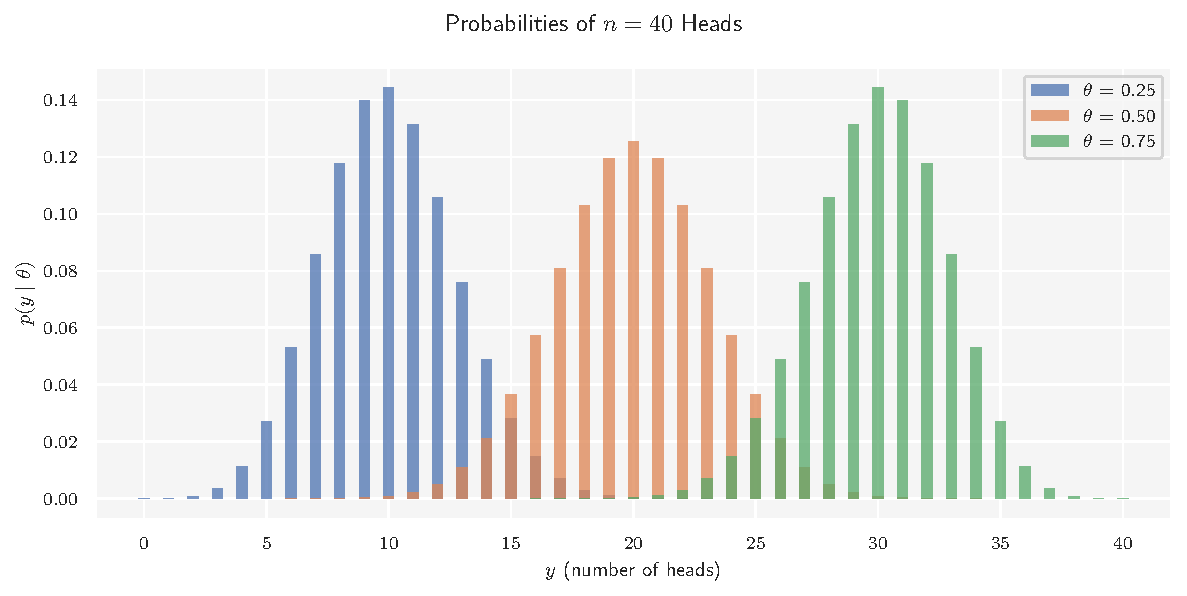
\includegraphics[scale=1]{binomial_distribution}
    \caption{Binomial distributions with $n=40$ coin flips and different success probabilities $\theta$. The coin is biased towards tails when $\theta < 0.5$ (blue) and heads when $\theta > 0.5$ (green). For $\theta=0.5$ (orange) the coin is unbiased (or fair). The legend indicates the values of the $\theta$.}
    \label{fig:binom_distribution}
\end{figure} 

If the value of $\theta$ is known, the binomial distribution tells us the expected distribution of heads. However, $\theta$ is an unknown model parameter, and thus we need to place a prior on it. For mathematical convenience, we choose a family of prior densities that lead to simple posterior densities. Considered as a function of $\theta$, \autoref{eq:coin_flip_likelihood} is of the form: 
\begin{equation*}
    \lhood \propto \theta^a \qty(1 - \theta)^b.
\end{equation*} 

If the prior density is of the same form, with its own parameterization of $a$ and $b$, then the posterior will also be of this form. Such a prior density can be parameterized as: 

\begin{equation*}
    \prior \propto \theta^{\alpha - 1} \qty(1 - \theta)^{\beta -1},
\end{equation*}

which is the beta distribution with shape parameters $\alpha>0$ and $\beta>0$. The parameters of the prior distribution are often called \textit{hyperparameters}. In order to ensure that the total probability is 1, the beta function,

\begin{equation*}
    B (\alpha, \beta) = \frac{\Gamma(\alpha)\Gamma(\beta)}{\Gamma(\alpha + \beta)},
\end{equation*}

where $\Gamma (z)$ is the gamma function, can be used as a normalizing constant:

\begin{equation}\label{eq:beta_prior}
    \prior = \frac{1}{B(\alpha, \beta)} \theta^{\alpha -1} (1-\theta)^{\beta -1}.
\end{equation}

The beta distribution is defined on the interval $[0, 1]$. \autoref{fig:beta_distribution} shows the beta distribution with different shape parameters. The figure displays the versatility of the beta distribution; the distribution adopts several shapes, determined by the shape parameters, including the uniform distribution with $\alpha = \beta = 1$. The uniform (blue) prior represents all the possible values for $\theta$ being equally likely a priori. The Gaussian-like (orange) prior is concentrated about $\theta=0.5$, and reflects a belief that the coin is equally probable to land heads or tails. The reverse J-shaped (green) prior is skewed towards a tail-biased outcome.

\begin{figure}[ht]
    \centering
    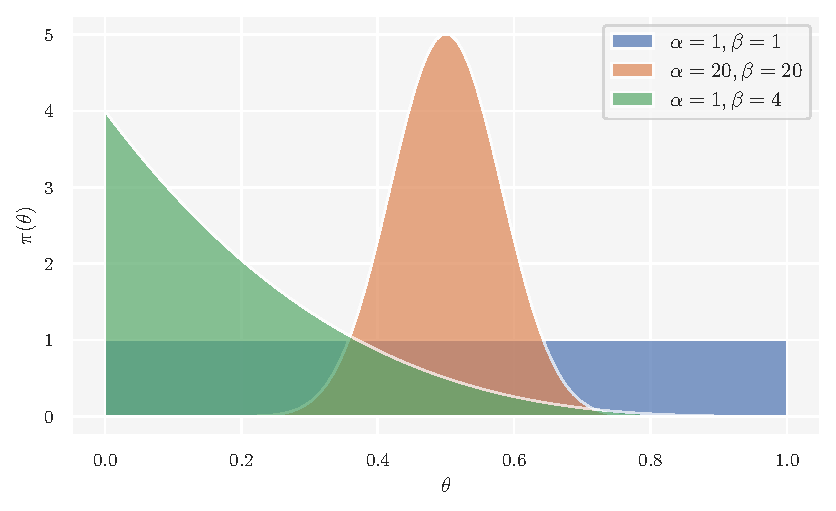
\includegraphics[scale=1]{beta_distribution}
    \caption{The beta prior probability distribution with different parameterizations by the two positive shape parameters. The beta distribution adopts several shapes controlled by the shape parameters; $\alpha=\beta=1$ gives a uniform distribution (blue), $\alpha=\beta=20$ gives a bell curve centered at $\theta=0.5$ (orange) and finally $\alpha=1$ and $\beta=2$ gives a reverse J-shaped distribution with a right tail (green).
    }
    \label{fig:beta_distribution}
\end{figure} 


Bayes' theorem, \autoref{eq:bayes_unnorm}, states that the posterior is proportional to the product of the likelihood and the prior. Thus, for our problem the posterior density for $\theta$ is given as: 

\begin{equation*}
    \pi (\theta \mid y) \propto \binom{n}{y} \theta^y (1-\theta)^{n-y} \frac{1}{B(\alpha, \beta)} \theta^{\alpha-1}(1-\theta)^{\beta -1}.
\end{equation*}

With fixed $n$ and $y$, the factor $\binom{n}{y}$ does not depend on the unknown parameter $\theta$, and neither does the beta function $B(\alpha, \beta)$. Thus can both be treated as constants when calculating the posterior distribution of $\theta$:

\begin{align*}
    \posterior &\propto \theta^y (1-\theta)^{n-y} \theta^{\alpha-1}(1-\theta)^{\beta -1} \\
    &= \theta^{\alpha + y -1} (1-\theta)^{\beta + n-y -1},
\end{align*}

or, more concisely:

\begin{equation}\label{eq:coin_posterior}
    \posterior \propto \theta^{\alpha' -1} (1-\theta)^{\beta' -1},
\end{equation}

with $\alpha'=\alpha+y$ and $\beta' = \beta + n - y$. We recognize that the expression above has the same functional form as the unnormalized beta distribution. The property that the posterior distribution follows the same parametric form as the prior distribution is called \textit{conjugacy}, and we say that the beta distribution is a \textit{conjugate prior} for the binomial likelihood.  

\autoref{fig:coin_flip_posterior} shows how the posteriors for the priors in \autoref{fig:beta_distribution} evolve as more and more data become available. For easier comparison, they have all been scaled vertically to have the same maximum value. \autoref{fig:coin_flip_posterior} clearly reveals the effect of the different priors; when there are few data, the shape of the posteriors vary in detail; as the number of data increases, the shape and location of the posteriors tend to converge and they all become sharply peaked. Since the priors reflect the different information or assumptions before the results, and the posteriors the updated knowledge in the light of data, this seems quite reasonable. If the data only are the outcome of a few flips, the analysis of these data is dominated by the prior information. However, as the data increases, the posterior is dominated by the likelihood and we are eventually led to the same conclusions regardless of our initial beliefs. In the limit of infinite data, all priors will provide the same posterior. From a practical point of view, we could obtain nearly indistinguishable posteriors for a finite amount of data. Thus, the choice of the prior becomes largely irrelevant given a sufficiently large amount of data.

\begin{figure}[H]
    \centering
    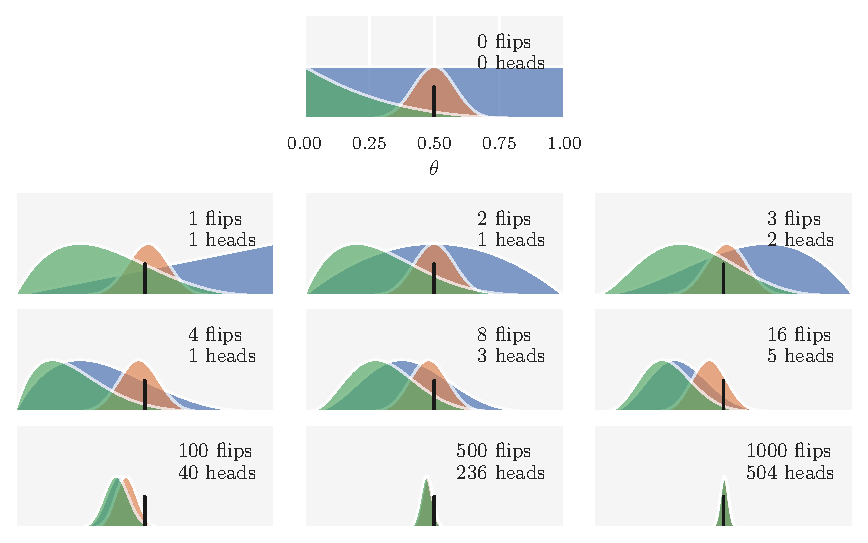
\includegraphics[scale=1]{coin_flip_posterior}
    \caption{The effect of different priors on the posterior as the number of data available increases. To aid in the comparison, they have all been scaled vertically to have the same maximum value. The number of data analyzed is indicated at the upper right-hand corner of each panel. In the first panel there are zero flips, and thus the densities represent the priors from \autoref{fig:beta_distribution}. The ground truth, $\theta=0.5$ (the coin is indeed fair), is indicated by the black vertical line. 
    }
    \label{fig:coin_flip_posterior}
\end{figure} 

 
Non-, weakly and informative priors. 

\url{http://www.stat.columbia.edu/~gelman/research/published/p039-_o.pdf}

An informative prior expresses specific, definite information about a variable. (then an example that I didn't understand).

An uninformative prior or diffuse prior expresses vague or general information about a variable. The term "uninformative prior" is somewhat of a misnomer. Such a prior might also be called a not very informative prior, or an objective prior, i.e. one that's not subjectively elicited. Uninformative priors can express "objective" information such as "the variable is positive" or "the variable is less than some limit".

%Two further curious points may be noted: (i) it takes quite a lot of flips to be able to estimate the bias-weighting with some degree of confidence (about a thousand to pin it down between 0.2 and 0.3); (ii) the posterior pdfs for the solid and dotted lines converge together quite quickly, but the dashed case takes much longer. The answer to the first observation is that it just does, but the number of flips required will depend on the actual bias-weighting of the coin. If the coin was tossed ten times and came up tails on every occasion, we would rapidly conclude that it was biased; on the other hand, the result of 45 heads and 55 tails in a hundred flips would still leave us somewhat uncertain as to whether the coin was fair. With regard to the second point, both the flat (solid) and the spiky (dotted) priors encode a large degree of ignorance about the nature of the coin. Despite the peculiar shape of the latter, it is fairly flat for most values of H; the strange-looking spikes at H = 0 and H = 1 disappear as soon as a head and a tail have been observed. The ‘fair-minded’ prior (dashed line), however, claims to be moderately well-informed about the character of the coin regardless of the data. It, therefore, takes much more to be convinced that the coin is not fair. Even though the prior probability for H = 0.5 was about a million times greater than that of H = 0.25, a thousand flips were enough to drag it (kicking and screaming, perhaps) to the conclusion that the value of H was less than 0.3 (but more than 0.2).

%non-, weakly and informative priors.

%These rules of thumb follow directly from the nature of the Bayesian analysis procedure:

%If the prior is uninformative, the posterior is very much determined by the data (the posterior is data-driven)

%If the prior is informative, the posterior is a mixture of the prior and the data

%The more informative the prior, the more data you need to "change" your beliefs, so to speak because the posterior is very much driven by the prior information

%If you have a lot of data, the data will dominate the posterior distribution (they will overwhelm the prior) 


\section{Bayesian Computation}

Move section to here?

As we saw in the previous section, conjugacy ensures analytic tractability. However, often the prior will not be the conjugate prior for the likelihood

In practice, ... not analytical

continuous data, normal model 

the derivation is quite tedious on the algebraic side, so we will here just provide the results and refer to ... for a full derivation.

...

where .. is the mean and .. the var. These are so-called summary statistics ... often used to derive

%================================================================
%\section{Gaussian Models and Posterior Checks}\label{sec:gaussian_models}
\section{Summarizing the Posterior}
%\section{Summarizing the Posterior}
%================================================================ 

The result of a Bayesian analysis is a posterior distribution which contains all the current information about the parameters $\theta$. 


In this section, we will look at both numerical and graphical ways to summarize the posterior:




\subsection{Posterior Plot}

In principle, the posterior distribution contains all the information about the possible parameter values. In practice, we must also present the posterior distribution somehow. If the examined parameter $\theta$
  is one- or two dimensional, we can simply plot the posterior distribution. Or when we use simulation to obtain values from the posterior, we can draw a histogram or scatterplot of the simulated values from the posterior distribution. If the parameter vector has more than two dimensions, we can plot the marginal posterior distributions of the parameters of interest.
  
 However, we often also want to summarize the posterior distribution numerically. The usual summary statistics, such as the mean, median, mode, variance, standard devation and different quantiles, that are used to summarize probability distributions, can be used. These summary statistics are often also easier to present and interpret than the full posterior distribution.

\subsection{Point estimates}

People often choose the median, just because it is more robust to outliers than the mean, or use the mean just because is a simple and familiar concept, or because they think their observable is truly the average of some process at some level, like molecules bouncing to each other or genes interacting with themselves and the environment.

Commonly used summaries of location are the mean, median and mode(s) of the distribution; variation is commonly summarized by the standard deviation, the interquartile range and other quantiles. Each summary has its own interpretation: for example, the mean is the posterior expectation of the parameter, and the mode may be interpreted as the single 'most likely' value, given the data (and the model).

\subsection{Posterior quantiles and intervals}




THIS IS NEW

The result of a Bayesian analysis is a posterior distribution, and all the information about the parameters given a dataset and a model is contained in the posterior distribution. Thus, by summarizing the posterior, we are summarizing the logical consequences of a model and data. A common practice is to report, for each parameter, the mean (or mode or median) to have an idea of the location of the distribution and some measure, such as the standard deviation, to have an idea of the dispersion and hence the uncertainty in our estimate. The standard deviation works well for normal-like distributions but can be misleading for other type of distributions, such as skewed ones. So, an alternative is to use the following measure.

\subsection{Posterior Predictive Check}

To make inferences about an unknown variable, often called predictive inferences, we follow a similar logic. Before the data $y$ are considered, the distribution of unknown but observable $y$ is 

\begin{equation}\label{eq:prior_predictive}
    \pi (y) = \int \lhood \prior \dd{\theta}
\end{equation}

%BDA, side 7

Posterior predictive check
Comparing the data to the posterior predictions of the model is called a posterior predictive check. When there appear to be systematic discrepancies that would be meaningful to address, you should consider expanding or changing the model so it may be a better description of the data.

One way to evaluate whether the least unbelievable parameter values are any good is via a posterior predictive check. A posterior predictive check is an inspection of patterns in simulated data that are generated by typical posterior parameters values. The idea of a posterior predictive check is as follows: If the posterior parameter values really are good descriptions of the data, then the predicted data from the model should actually “look like” real data. If the patterns in the predicted data do not mirror the patterns in the actual data, then we are motivated to invent models that can produce the patterns of interest.

---

Posterior Predictive Distributions
For evaluating the fit of a model, perhaps the most flexible approach is to examine the Bayesian posterior predictive distribution. The posterior predictive distribution is the distribution of future observable data, based on the posterior distribution. It is defined as: 

eq same as 6.1 in BDA 

In this equation, $y_{rep}$ is future data that could be drawn from the posterior distribution, $y$ is the current data, and $\theta$ is the model parameter. Notice that the last two terms (prior to $d\theta$) are the posterior density for the parameter. The first term is the sampling density for future data, conditional on the parameter. This equation simply specifies a form for the distribution of future data, given the model parameter and data. If a model fits the current data well, then we expect that simulated future data should look much like the current data. Thus, we can simulate data from the posterior predictive distribution, compare it to the observed data, and determine whether the model has an appropriate fit. 

---

Following the same logic, prior predictive distribution  


\subsection{Measures of Predictive Accuracy}

Goodness of fit in Bayesian analyses is routinely assessed using a method referred to as the ‘Bayesian p-value’ and posterior predictive checks (Gelman et al., 1996).

s. 166/167 i BDA 

%================================================================
%\section{Gaussian Models and Posterior Checks}\label{sec:gaussian_models}
\subsection{Bayesian Analysis}
%\section{Summarizing the Posterior}
%================================================================


Posterior - all information

We will use a Gaussian model with unknown mean and variance to illustrate the following, since it is continuous and

The Bayesian Toolkit

One point that must be clear from the beginning is that the Bayesian approach is a complete inferential approach. Therefore, it covers confidence evaluation, testing, prediction, model checking, and point estimation. We will progres- sively cover the different facets of Bayesian analysis in other chapters of this book, but we address here the issue of confidence intervals because it is rather a straightforward step from point estimation.

normal models important blabla

As we saw in the previous section, conjugacy ensures tractable posteriors. Sufficent summary statistics, (mean and variance for normal)

The derivation requires some tedious algebra, so we simply state the result (Murphy, 07)

\url{https://en.wikipedia.org/wiki/Conjugate_prior#When_likelihood_function_is_a_continuous_distribution}


The comprehensive derivation can be found in appendix B. 

Devore, p. 781 

Note that the posterior mean $\mu_0'$ is a weighted average of the prior mean $\mu_0$ and the data mean $\bar{x}$, with weights that are the reciprocals of the prior variance and the variance of $\bar{x}$. It makes sense to define the \textbf{precision} as the reciprocal of the variance because a lower variance implies a more precise measurement and the weights then are the corresponding precisions. Furthermore, the posterior variance is the reciprocal of the sum of the reciprocals of the two variances, but this can be described much more simply by saying that the posterior precision is the sum of the prior precision plus the precision of $\bar{x}$.  


Sufficient statistics are useful in algebraic manipulations of likelihoods and posterior distributions.

sufficient summary statistics, lfi for cogsci, side 16, Fisher-Neyman Factorization Theorem

\url{https://bookdown.org/mrwhalen/bayes_book/summarizing-posterior-distributions.html}

Summarizing Posterior Distributions
Obtaining a posterior distribution is great, but does not provide us with much concrete to discuss or convey to others. Therefore, we need ways to distill the distribution into point estimates, or summary statistics. The most common summary statistics for posterior distributions will be the posterior mean, posterior mode and posterior median.

At times, there will be different reasons to use each summary statistic, but most often a safe assumption is to report the posterior mean $\pm$ posterior standard devition.

From a decision theory standpoint there technically are mathematical ways to determine which point estimate is the best to use in certian instances, but that is beyond the scope of this tutorial. However, here are the answers that come from magic (maybe I will post the proofs in the appendix:

1. If the loss function is quadratic, the best estimate is the posterior mean.
2. If the loss function is an absolute loss, the best estimate is the posterior median.
3. If the loss function is an All-or-nothing loss, the best estimate is the posterior mode

The posterior mode is just the expected value of the parameter estimate, using the posterior distribution.

Recall that a mode is simply the most frequent point in a data set. In a Bayesian distribution, this refers to the peak of the distribution (the parameterestimate with the highest overall weight). 

The posterior median refers to the value which divides the distribution in half. This is a bit more challenging to calculate by hand (and is the least frequently used summary statistic) but it is worth seeing where this value comes from.

We need to find the value $\theta$ which has 50\% of the probability to the left and 50\% to the right. It is also worth noting that the median is tricky to calculate for discrete distributions (hence why it is rarely seen).


Credible Intervals

There is a lot to say about the difference between Bayesian Credible Intervals and Classical Confidence Intervals. I will avoid this entire discourse and just say that in Bayesian statistics a Credible Interval is the interval in which we have a 95\% probabilistic belief the parameter is in that interval.

In Chapter 1, Thinking Probabilistically, we introduced the concept of posterior predictive checks, and, in subsequent chapters, we have used it as a way to evaluate how well models explain the same data that's used to fit the model. The purpose of posterior predictive checks is not to dictate that a model is wrong; we already know that! By performing posterior predictive checks, we hope to get a better grasp of the limitations of a model, either to properly acknowledge them, or to attempt to improve the model. Implicit, in the previous statement is the fact that models will not generally reproduce all aspects of a problem equally well. This is not generally a problem given that models are built with a purpose in mind. A posterior predictive check is a way to evaluate a model in the context of that purpose; thus, if we have more than one model, we can use posterior predictive checks to compare them.

%================================================================
%\section{Summarizing the Posterior}
%================================================================

In Bayesian inference, posterior beliefs about parameters are updated according to \textit{Bayes' theorem} upon observing data.  

The mean of this posterior distribution gives a point estimate of $\theta$. 

An interval having a posterior probability $.95$ gives a $95\%$ \textit{credibility} interval, an interval within which an unobserved parameter value falls with a particular probability, the Bayesian analogue of a $95\%$ confidence interval \cite[p. 777]{STK}.

Credible intervals 

HDI 

Energy

- mean, median, mode: point estimates

- variance and standard deviation: spread -> uncertainty 

- credible intervals, highest density posterior (hdp) 


RMSE, true value, SEM 

In practice, we generally do not have the value of the true parameter $\theta$ at hand. Instead, we have an estimation in the form of a posterior distribution. Thus, what we can do is find out the value of $\hat{\theta}$ that minimizes the expected loss function. By expected loss function, we mean the loss function averaged over the whole posterior distribution. 

%================================================================
%\subsubsection{With Unknown Mean and Variance}
%================================================================

%The comprehensive derivation can be found in appendix B. 




%================================================================
%\section{The Influence of the Prior and How to Choose One}\label{sec:prior}
%================================================================

%\url{http://www.stat.columbia.edu/~gelman/research/published/p039-_o.pdf}

%\begin{itemize}
%    \item Flat
%    \item Uninformative
%    \item Diffuse
%    \item The Jeffreys’ Prior: Suppose we cannot easily find the natural scale on which the likelihood is in data-translated format, or that such a decomposition does not exist. Jeffreys (1961) proposed a general prior in such cases, based on the Fisher information I of the likelihood. 
%    \item When a prior distribution is not integrable it is said to be \textit{improper}
%\end{itemize}


%================================================================
%\subsection{Conjugate Prior Distributions}
%================================================================

%In Bayesian probability theory, if posterior distributions are in the same family as the prior distributions, then both prior and posterior are called conjugate distributions and the prior is called conjugate prior.

%Conjugacy is formally defined as follows. If $\mathcal{F}$ is a class of sampling distributions $p \left(y | \theta \right)$, and $\mathcal{P}$ is a class of prior distributions for $\theta$, then the class $\mathcal{P}$ is \textit{conjugate} for $\mathcal{F}$ if

%\begin{equation}
%    \pi \left(\theta | y \right) \in \mathcal{P} \, \forall p \left(\cdot | \theta \right) \in \mathcal{F} \land \pi (\cdot) \in \mathcal{P}
%\end{equation}

%This definition is formally vague since if we choose $\mathcal{P}$ as the class of all distributions, then $\mathcal{P}$ is always conjugate no matter what class of sampling distributions is used. We are most interested in \textit{natural} conjugate prior families, which arise by taking $\mathcal{P}$ to be the set of all densities having the same functional form as the likelihood \cite{ABC_ch1}.

%A conjugate prior of a likelihood is a prior that, when used in combination with a given likelihood, returns a posterior with the same functional form as the prior. cite BAP

%================================================================
%\section{Prior and Posterior Predictive Checks}
%================================================================

%\begin{itemize}
    %\item \url{https://docs.pymc.io/notebooks/posterior_predictive.html}
    %\item \url{https://avehtari.github.io/masterclass/slides_ppc.pdf}
    %\item \url{https://vasishth.github.io/bayescogsci/book/sec-priorpred.html}
    %\item \url{https://betanalpha.github.io/assets/case_studies/principled_bayesian_workflow.html#113_Prior_Predictive_Checks}
    %\item \url{http://bebi103.caltech.edu.s3-website-us-east-1.amazonaws.com/2018/tutorials/t6a_model_generation_and_prior_predictive_checks.html} python
%\end{itemize}

%================================================================
%\section{Uncertainty/Sensitivty Analysis in the Bayesian Paradigm}
%================================================================






%================================================================
%\subsection{The Prior and Posterior Predictive Distributions}\label{sec:predictive}
%================================================================

%BDA, side 7





%================================================================
%\section{Why Bayes?}
%================================================================

%End chapter with this? No, move to introduction
